% !TEX TS-program = pdflatex

\documentclass[unicode,11pt,notheorems,xcolor=table]{beamer}

\usepackage[T2A]{fontenc}
\usepackage[utf8]{inputenc}
\usepackage[russian]{babel}
\usepackage{amsmath,amsfonts,amssymb,amsthm}
\usepackage{mathtools}
\usepackage{diagbox}

\usepackage{ulem}
\usepackage{tikz, graphicx}
%\usepackage{tkz-graph}
\usetikzlibrary{matrix,arrows,decorations.pathmorphing, arrows.meta,positioning}
\usetikzlibrary{positioning,calc}
\usetikzlibrary{petri}
\usetikzlibrary{decorations.pathreplacing}

%Описание стиля презентации
\usetheme[sidebar=0]{kfmn} 
\setbeamercovered{transparent}

%\definecolor{cyan}{RGB}{240,217,1}
%\definecolor{vgugreen}{RGB}{143,188,103}
%\definecolor{vgured}{RGB}{234,38,40}
%\definecolor{vgublue}{RGB}{53,101,167}
\hypersetup{colorlinks,linkcolor=,urlcolor=blue}

\makeatletter
	\g@addto@macro{\endtabular}{\rowfont{}}% Clear row font
	\makeatother
	\newcommand{\rowfonttype}{}% Current row font
	\newcommand{\rowfont}[1]{% Set current row font
		\gdef\rowfonttype{#1}#1\ignorespaces%
	}
\makeatother

\newcommand{\myunit}{9mm}
\tikzset{
    node style sp/.style={draw,circle,minimum size=\myunit},
    node style ge/.style={circle,minimum size=\myunit},
    arrow style mul/.style={draw,sloped,midway,fill=white},
    arrow style plus/.style={midway,sloped,fill=white},
}

%[0, 6, 8, 8, 10, 5, 6, 10, 8, 10, 10], 

\pgfdeclareimage[height=8mm]{university-logo}{logo-iem.png}
\logo{\pgfuseimage{university-logo}}
%2[0, 11, 10, 8, 11, 5, 11, 11, 8, 11, 10, 11],

\titlepicture{
	\begin{tikzpicture}[y=1.4cm,overlay,rotate=8]
	\coordinate (O) at (-3cm,0.9cm);
	\filldraw[thick,draw= vgublue, fill=vgublue!20!white] (0,0) circle[radius=4.2cm];
	\clip (0,0) circle[radius=4.2cm];
	\draw (-1.5,1.5) node{
	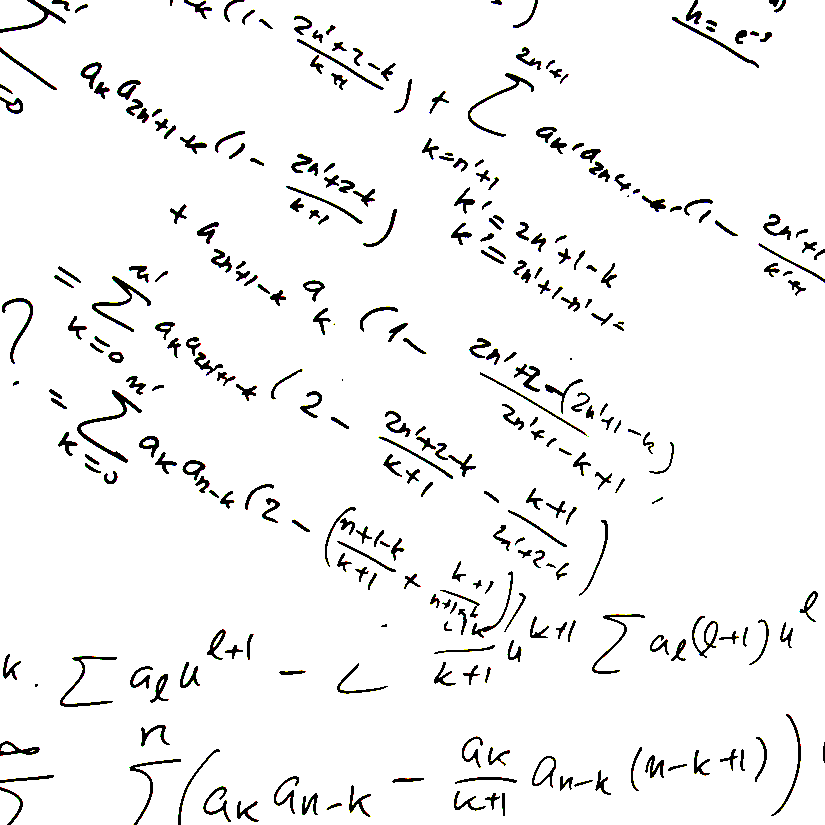
\includegraphics[width=8cm]{titlepic.png}
	};
\end{tikzpicture}
}

\usepackage[math]{iwona}

\newcommand{\hplus}{\mathbin{\hat+}}
\newcommand{\hdot}{\mathbin{\hat\cdot}}
% Описание теорем
\newtheorem{theorem}{Теорема}
\newtheorem{seq}{Следствие}
%%

\LECT % 

% Титульный лист теорем
\author[Д.\,В. Чупраков]{канд.\,физ.-матем.\,наук, доцент Д.\,В. Чупраков\\[6pt] usr10381@vyatsu.ru}

\institute[ВятГУ]{ФГБОУ ВО Вятский государственный университет}

\department{Факультет экономики и финансов}

\title[Лекция~13. Случайные события и вероятности]{
	Введение в экономико-математическое моделирование\\[12pt]
	Лекция~12. Случайные события и вероятности}
\subtitle{Формула Байеса и повторение испытаний}
\date{25 ноября 2020~г.}


\setbeamercovered{invisible}

\setbeamercolor{math text}{fg=vgured!70!black}


\begin{document}


\maketitle

\begin{frame}{Структура лекции}
	\tableofcontents
\end{frame}

\section{Формула Байеса}

\subsection{Понятие полной вероятности}
\begin{frame}{Полная группа событий}{}
    \begin{block}{}
        События $H_1, H_2,\ldots, H_n$ образуют \alert{полную группу событий}, если 
        \begin{enumerate}
            \item события \alert{$H_1, H_2,\ldots, H_n$} попарно \underline{несовместны};
            \item \alert{$H_1+H_2+\ldots+H_n = 1$}
        \end{enumerate}
    \end{block}

    \bigskip
    \begin{itemize}
        \item События образуют полную группу, если в результате опыта происходит ровно одно из них.
        \item Все исходы опыта образуют полную группу событий.
        \item Событие $A$ и противоположное к нему событие $\overline{A}$ образуют полную группу событий.
    \end{itemize}
\end{frame}

\begin{frame}{Полная вероятность}
    Следствием теорем о вероятностях   является формула полной вероятности:
    \begin{theorem}{}
        Если 
        \begin{itemize}
            \item $H_1,H_2,\ldots, H_n$~--- полная группа событий;
            \item известны условные вероятности $p(A/H_i)$ для всех $i\in \{1,2,\ldots,n\}$,
        \end{itemize}
        то
        $$
           \alert{p(A) = \sum_{i=1}^n p(H_i)p(A/H_i) =p(H_1)p(A/H_1)+ \ldots+p(H_n)p(A/H_n)}
        $$
    \end{theorem}
\end{frame}
\begin{frame}[allowframebreaks]{Типовой пример. Полная вероятность}
    \begin{exampleblock}{}
        В магазин поступила новая продукция с трех предприятий. Процентный состав этой продукции следующий: $20\%$ ~--- продукция первого предприятия, $30\%$~--- продукция второго предприятия, $50\%$~--- продукция третьего предприятия; 
        Вероятность брака продукции первого предприятия~--- $1\%$, второго предприятии - $0.5\%$, третьего~--- $2\%$. Найти вероятность того, что случайно купленная новая продукция окажется бракованной.    
    \end{exampleblock}
    \begin{itemize}
    
        \item[] \structure{Формализуем задачу:}
        \item Событие $A$~--- товар бракованный. Может наступить только с одним из несовместных событий $H_1$, $H_2$, $H_3$:
        \begin{tabular}{l@{\;---\;}l@{,\quad}l@{,\quad}l}
            $H_1$ & продукт 1 предприятия & $p(H_1)=0.2$ &$p(A/H_1)=0.01$\\
            $H_2$ & продукт 2 предприятия & $p(H_2)=0.3$ & $p(A/H_2)=0.005$\\
            $H_3$ & продукт 3 предприятия & $p(H_3)=0.5$ & $p(A/H_3)=0.02$\\
        \end{tabular}
        \item $p(H_1)+p(H_2)+p(H_3)=1$~--- это полная группа событий.
        \item Применим формулу полной вероятности
        \begin{multline*}
            p(A)= p(H_1)p(A/H_1)+p(H_2)p(A/H_2)+p(H_3)p(A/H_3)
            =\\
            = 0.2\cdot 0.01+ 0.3\cdot 0.005+ 0.5\cdot 0.02 
            = 0.0135
        \end{multline*}
        \item 
        Итак, $p(A)=0.0135$ или $1.35\%$.
    \end{itemize}
    
\end{frame}

\subsection{Формула Байеса}
\begin{frame}[allowframebreaks]{Формула Байеса}
    \begin{itemize}
        \item Предположим, есть полная группа событий $H_1,H_2, \ldots, H_n$ , вероятности которых известны и равны $p(H_1), p(H_2),\ldots, p(H_n)$.
        \item Назовем эти события \alert{гипотезами}
        \item Пусть некоторое случайное событие $A$ может произойти, только если осуществится одна из этих гипотез $H_i$. Причём известны вероятности $p(A/H_i)$
        \item На основании формулы полной вероятности 
        $$
            p(A) = p(H_1)p(A/H_1)+ p(H_2)p(A/H_2)+\ldots+ p(H_n)p(A/H_n)
        $$
        \framebreak
        \item Произведено испытание, в результате которого произошло событие~$A$. 
        \item 
        Возникает вопрос, какова вероятность, что при этом осуществилась одна из гипотез: $H_1$, $H_2$, \ldots, $H_n$? То есть интересует $p(H_i/A)$.

        \item Посмотрим на вероятность появления события $H_i\cdot A$.
        
        $$
            p(H_i\cdot A) = p(H_i)p(A/H_i)= p(A)p(H_i/A)
        $$
        
        \item Выразим $p(H_i/A)$:
        $$
            p(H_i/A) = \frac{p(H_i)p(A/H_i)}{p(A)}
        $$
    \end{itemize}

    Итак, имеет место теорема:

    \begin{theorem}[Байеса]
        Если 
        \begin{itemize}
            \item $H_1,H_2,\ldots, H_n$~--- полная группа событий;
            \item  известны вероятности $p(H_i)$ для всех $i\in \{1,2,\ldots,n\}$,
            \item известны условные вероятности $p(A/H_i)$ для всех $i\in \{1,2,\ldots,n\}$,
        \end{itemize}
        то
        $$
            p(H_i/A) = \frac{p(H_i)p(A/H_i)}{\sum_{j=1}^n p(H_j)p(A/H_j)}
        $$
    \end{theorem}
 \end{frame}

 \begin{frame}[allowframebreaks]{Типовой пример. Формула Байеса}{}
    \begin{exampleblock}{}
        Допустим у меня есть комплект \texttt{D\&D} дайсов. Я беру 3 кости: с 4, 6 и 8 гранями. Подбрасываю какую-то из них и говорю вам, что выпало 2. Какую кость я~подбрасывал?
    \end{exampleblock}
    \framebreak
    \begin{itemize}
        \item \structure{Формализуем:} событие $A$~--- выпала 2 могло произойти, в одном из трех случаев:
        \begin{tabular}{l@{\;---\;}l@{,\quad}l@{,\quad}l}
            $H_1$ & выбран D3 & $p(H_1)=1/3$ &$p(A/H_1)=1/3$\\
            $H_2$ & выбран D6 & $p(H_2)=1/3$ & $p(A/H_2)=1/6$\\
            $H_3$ & выбран D8 & $p(H_3)=1/3$ & $p(A/H_3)=1/8$\\
        \end{tabular}
        \item Это априорные --- доопытные вероятности
        \item \structure{Найдем вероятность $A$} по формуле полной вероятности:
        
        \begin{multline*}
            p(A)
            =p(H_1)p(A/H_1) + p(H_2)p(A/H_2) + p(H_3)p(A/H_3) 
            =\\
            =\frac{1}{3}\cdot \frac{1}{3} + \frac{1}{3}\cdot \frac{1}{6}+ \frac{1}{3}\cdot \frac{1}{8} = \frac{5}{24}.
        \end{multline*}
        \item Применим теперь \structure{формулу Байеса:}
        
        \begin{align*}
            p(H_1/A) &= \frac{p(H_1)\cdot p(A/H_1)}{p(A)} = \frac{1/3\cdot 1/3}{5/24} = \frac{8}{15} \approx 0.53.\\
            p(H_2/A) &= \frac{p(H_2)\cdot p(A/H_2)}{p(A)} = \frac{1/3\cdot 1/6}{5/24} = \frac{4}{15} \approx 0.27.\\
            p(H_3/A) &= \frac{p(H_3)\cdot p(A/H_3)}{p(A)} = \frac{1/3\cdot 1/8}{5/24} = \frac{1}{5} \approx 0.20.
        \end{align*}
            
        \item Итак, я бросал 
        \begin{itemize}
            \item D3 с вероятностью $53\%$,\\
            \item D6~--- с вероятностью $27\%$,
            \item D8~--- с вероятностью $20\%$.
        \end{itemize}
        
        \hrule
        
        \medskip
        Знание результата существенно изменило оценку действий.
        
    \end{itemize}
 \end{frame}

\begin{frame}[allowframebreaks]{Пример на злобу дня}
    \begin{exampleblock}{}
        Есть некоторое заболевание на К, которое диагностируют у 3\% процентов населения страны. Экспресс-тест на вирусную РНК дает верные результаты в 94\% случаев. Какова вероятность оказаться заболевшим, если тест показывает положительный результат?
    \end{exampleblock}
    \begin{itemize}
        \item \structure{Формализуем:} событие $A$~--- Тест показал положительный результат  могло произойти, вместе со следующими событиями:
        \begin{tabular}{l@{\;---\;}l@{\quad}l@{,\quad}l}
            $H_1$ & пациент болен    & $p(H_1)=0.03$ &$p(A/H_1)=0.94$\\
            $H_2$ & пациент не болен & $p(H_2)=0.97$ & $p(A/H_2)=0.06$\\
        \end{tabular}
        \item \structure{Полная вероятность $A$}~--- положительного результата теста равна:
            \begin{multline*}
                p(A)
            =p(H_1)p(A/H_1) + p(H_2)p(A/H_2)
            =\\
            =0.03\cdot 0.94+0.97\cdot 0.06 = 0.0864.
        \end{multline*}
        \item Применим теперь \structure{формулу Байеса} чтобы определить, вероятность болезни у пациента:
        \begin{multline*}
            p(H_1/A) = \frac{p(H_1)\cdot p(A/H_1)}{p(A)} = \frac{0.03\cdot 0.94}{0.0864}  \approx 0.326.
        \end{multline*}
    \end{itemize}
    
    \medskip
    \hrule
    \medskip

    Итак, вероятность того, что пациент действительно болен не~больше $33\%$.

    \framebreak
    \begin{exampleblock}{}
        Тест проведен еще раз и снова получен положительный результат. Какова теперь вероятность оказаться заболевшим
    \end{exampleblock}
    \begin{itemize}
        \item Вновь событие $A$~--- положительный результат теста, но априорные вероятности событий изменились:
        \begin{tabular}{l@{\;---\;}l@{\quad}l@{,\quad}l}
            $H_1$ & пациент болен    & $p(H_1)=0.33$ &$p(A/H_1)=0.94$\\
            $H_2$ & пациент не болен & $p(H_2)=0.67$ & $p(A/H_2)=0.06$\\
        \end{tabular}
        \item Полная вероятность $A$~--- положительного результата теста равна:
    
        \begin{multline*}
            p(A)
            =p(H_1)p(A/H_1) + p(H_2)p(A/H_2)
            =\\
            =0.33\cdot 0.94+0.67\cdot 0.06 
            = 0.3504.
        \end{multline*}
        \item Применим теперь \structure{формулу Байеса} чтобы определить, вероятность болезни у пациента:
        \begin{multline*}
            p(H_1/A) = \frac{p(H_1)\cdot p(A/H_1)}{p(A)} = \frac{0.33\cdot 0.94}{0.3504}  \approx 0.885
        \end{multline*}
    \end{itemize}
    
    \medskip
    \hrule
    \medskip
    
    Итак, вероятность того, что пациент действительно болен после двухкратного положительного результата теста равна $89\%$.
\end{frame}






\begin{frame}{}
    \begin{alertblock}{}
        Многократно применяемая формула Байеса~--- мощный инструмент принятия решений.
        Она позволяет последовательно уточнять вероятности гипотез о развитии управляемой системы в зависимости от события, возникающих при функционировании  этой системы.
    \end{alertblock}
\end{frame}
\section{Повторение испытаний}
\begin{frame}{Задача повторения испытаний}{}
    % Поставим задача, вычислить 

    Допустим, 
    \begin{itemize}
        \item Испытания независимы~--- появление события не влияет на вероятность появления события при следующих опытах.
        \item Вероятность $p=p(A)$ появления события $A$ одинакова в каждом их опытов.
        \item Вероятность противоположного события $q=p(\overline{A})=1-p$.
        \item \structure{Требуется} найти вероятность $P_n(k)$~--- наступления события $A$  ровно $k$ раз из $n$ проведенных опытов.
    \end{itemize}
    

    В этом случае говорят, что поставлена \alert{задача повторения независимых испытаний.}

    Искомая вероятность обозначается $P_n(k)$.
\end{frame}
\begin{frame}{Вероятность появления заданного числа событий}{}
    
    \begin{enumerate}
        \item По теореме о произведении независимых событий:
        $$
            P(\underbrace{A\cdot A}_k \underbrace{\overline{A} \cdot \overline{A}}_{n-k})= p^k q^{n-k}.
        $$
        \item Теперь заметим, что выбрать $k$ испытаний, в которых произошло событие можно~$C_n^k = \frac{n!}{k!(n-k)!}$ способами, при этом все эти события несовместны.
        \item  По теореме о сумме несовместных событий
        $$
            P_n(k)= \underbrace{p^k q^{n-k} + \ldots + p^k q^{n-k}}_{C_n^k}  = C_n^k p^k q^{n-k}. 
        $$


    \end{enumerate}
\end{frame}

\subsection{Формула Бернулли}

\begin{frame}{Формула Бернулли}{}
    \begin{block}{Формула Бернулли}
        \itshape
        Вероятность того, что при $n$ независимых испытаниях событие~$A$ осуществится ровно $k$ раз равна
        $$
            P_n(k)= C_n^k p^k q^{n-k}. 
        $$
    \end{block}
\end{frame}
    

\begin{frame}{Пример. Формула Бернулли}{}

\end{frame}

\begin{frame}{Неприменимость формулы Бернулли}{}
    Формула требует выполнения действий над громадными числами, поэтому пользоваться формулой Бернулли при больших значениях $n$ достаточно сложно.
\end{frame}
\subsection{Локальная теорема Муавра\,---\,Лапласа}

\begin{frame}{Локальная теорема Муавра\,---\,Лапласа}{}
    \begin{itemize}
        \item Нельзя ли вычислить интересующую нас вероятность, не прибегая к формуле Бернулли? 
        \item Да, можно, приближенно!
        \item Для этого используется функция Гаусса:
        $$
             \varphi(x)= \frac{1}{\sqrt{2\pi}} e^{-\frac{x^2}{2}}
        $$
    \end{itemize}
   
    \begin{block}{Локальная теорема Муавра\,---\,Лапласа}
        \itshape
        Если вероятность $p=p(A)$ в каждом испытании постоянна и~$p\neq 1$, $p \neq 0$, то вероятность $P_n(k)$ того, что событие $A$ появится в $n$ испытаниях ровно $k$ раз приближенно равна
        $$
            P_n(k) \approx \frac{1}{\sqrt{npq}} \varphi(x), \quad\text{при}\quad x = \frac{k-np}{\sqrt{npq}}
        $$  

    \end{block}
\end{frame}
\begin{frame}{Вычисление функции Гаусса}{}
    Для вычисления функции Гаусса 
    $$
        \varphi(x)= \frac{1}{\sqrt{2\pi}} e^{-\frac{x^2}{2}}
    $$
    рекомендуется использовать:
    \begin{itemize}
        \item \href{https://cloud.mail.ru/public/5oAx/3MrM7rR4E}{таблицы} значений.
        \item функции электронных таблиц:
        \begin{itemize}
            \item \texttt{=ФИ(x)} \hfill (MS Excel , LibreOffice Calc)
            \item \texttt{=НОРМ.СТ.РАСП(x;0)} \hfill (MS Excel 2010, LibreOffice Calc)
            \item \texttt{=PHI(x)} \hfill (Google spreadsheets)
        \end{itemize}
        \end{itemize}
    \begin{block}{Свойство четности функции Гаусса}
        $\varphi(-x)=\varphi(x)$
    \end{block}
\end{frame}

\begin{frame}{Типовой пример}{}
    \begin{exampleblock}{Задача}
        Найти вероятность того, что при $400$ испытаниях событие наступит ровно $104$ раза, если вероятность его появления в каждом испытании равна $p=0.2$.
    \end{exampleblock}
    \begin{itemize}
        \item Исходные данные:
        $
            n=400, \quad k=104,  \quad p=0.2,  \quad q=1-p =0.8
        $
        \item $n$~--- большое, воспользуемся локальной теоремой Муавра\,---\,Лапласа.
        \item Вычислим $\sqrt{npq}= \sqrt{400 \cdot 0.2 \cdot 0.8} =\sqrt{64}=8$
        \item Вычислим $x = \frac{k-np}{\sqrt{npq}} = \frac{104-400 \cdot 0.2}{8} =\frac{24}{8}=3 $
        \item Вычислим  $\varphi(x)= \varphi(3) \approx 0.0044$\hfill \texttt{=ФИ(3)}
        \item  $        P_{400}(104) \approx \frac{1}{\sqrt{npq}} \varphi(x)  \approx \frac{1}{8} 0.0044 \approx 0.00055$
    \end{itemize}
    \structure{Ответ:} вероятность $P_{400}(104) \approx 0.00055$.
\end{frame}
\begin{frame}{Проблема}
    \begin{block}{Странная ситуация}
        При проведении рекламной кампании на проспекте был размещен рекламный стенд.
        Ежедневно его видят $5000$ человек. Вероятность того, что человек среагирует на рекламу равна $0.1$. Руководство интересует, вероятность того, что за месяц (30~дней) на рекламу среагируют ровно $15782$~человека?        
    \end{block}
    \pause
    \begin{itemize}
        \item Точное значение числа появлений события чаще всего не информативно.
        \pause
        \item При увеличении числа испытаний $n$ вероятность того, что произойдет ровно $k$ событий стремится к нулю. 
        \pause
        \item Интереснее какова вероятность, что число событий окажется в промежутке $k_1 \leqslant k \leqslant k_2$
    \end{itemize}

\end{frame}


\subsection{Интегральная теорема Муавра\,---\,Лапласа}

\begin{frame}{Интегральная теорема Муавра\,---\,Лапласа}{}
   
    \begin{block}{Интегральная теорема Муавра\,---\,Лапласа}
        \itshape
        Если вероятность $p=p(A)$ в каждом испытании постоянна и~$p\neq 1$, $p \neq 0$, то вероятность $P_n(k_1,k_2)$ того, что событие $A$ появится в $n$ испытаниях  от $k_1$ до $k_2$ раз приближенно равна определенному интегралу
        $$
            P_n(k_1,k_2) \approx \int\limits_{x_1}^{x_2}\varphi(x)dx, 
        $$
        где
        $$  
            x_1 = \frac{k_1-np}{\sqrt{npq}},\quad x_2 = \frac{k_2-np}{\sqrt{npq}}
        $$  

    \end{block}
\end{frame}
\begin{frame}{Интегральная теорема Муавра\,---\,Лапласа}{}
    Рассмотрим функцию Лапласа
    $$
        \Phi(x) = \int\limits_0^x \varphi(z)dz = \frac{1}{\sqrt{2\pi}}\int\limits_0^x e^{-\frac{z^2}{2}}dz
    $$
    \begin{block}{Интегральная теорема Муавра\,---\,Лапласа}
        \itshape
        Если вероятность $p=p(A)$ в каждом испытании постоянна и~$p\neq 1$, $p \neq 0$, то вероятность $P_n(k_1,k_2)$ того, что событие $A$ появится в $n$ испытаниях  от $k_1$ до $k_2$ раз приближенно равна определенному интегралу
        $$
            P_n(k_1,k_2) \approx \Phi(x_2)-\Phi(x_1)
        $$
        где
        $x_1 = \dfrac{k_1-np}{\sqrt{npq}},\quad x_2 = \dfrac{k_2-np}{\sqrt{npq}}$  

    \end{block}
\end{frame}

\begin{frame}{Вычисление функции Лапласа}{}
    Функция Лапласа (интеграл Гаусса)
    $$
        \Phi(x) = \frac{1}{\sqrt{2\pi}}\int\limits_0^x e^{-\frac{z^2}{2}}dz
    $$
    не берущийся интеграл.

    \bigskip

    При решении задач пользуются специальной таблицей значений или функциями электронных таблиц

    \begin{itemize}
        \item В \href{https://cloud.mail.ru/public/3hfk/5Ey4LLdoi}{таблице} присутствуют значения $\Phi(x)$ для $0\leqslant x \leqslant 5$.
        \begin{itemize}
            \item если $x<0$,  то $\Phi(x)= -\Phi(-x)$\hfill \structure{Функция $\Phi(x)$~--- нечетная;}
            \item если $x>50$, то $\Phi(x)= 0.5$;
        \end{itemize}
        \item функции электронных таблиц:
        \begin{itemize}
            \item \texttt{=ГАУСС(x)} \hfill (MS Excel , LibreOffice Calc)
            \item \texttt{=GAUSS(x)} \hfill (Google Sheets)
        \end{itemize}
        \end{itemize}
\end{frame}

\begin{frame}{}
\end{frame}

\subsection{Оценка отклонения частоты от вероятности}
\begin{frame}[allowframebreaks]{Отклонение частоты от вероятности}{}
    Поставим перед собой задачу:
    \begin{block}{}
        Найти вероятность того, что отклонение относительной частоты $\frac{k}{n}$ от постоянной вероятности $p$ по абсолютной величине не превышает заданного числа $\Delta>0$:
    \qquad$ p\Big( \big|\tfrac{k}{n} - p \big| \leqslant \Delta \Big)$
    \end{block}
    \begin{itemize}
        \item Преобразуем неравенство:
        \begin{gather*}
            \left| \frac{k}{n} - p \right| \leqslant \Delta\\
            -\Delta \leqslant \frac{k}{n} - p \leqslant \Delta\\
            -\Delta n \leqslant k - pn \leqslant \Delta n\\
            pn-\Delta n \leqslant k \leqslant pn+\Delta n
        \end{gather*}
        \item Оценим вероятность
        \begin{multline*}
            p\Big( \big|\tfrac{k}{n} - p \big| \leqslant \Delta \Big) 
            = p\Big( pn-\Delta n \leqslant k \leqslant pn+\Delta n \Big) 
            =\\
            = P_n(pn-\Delta n, pn+\Delta n) 
        \end{multline*}
         \item Применим интегральную теорему Муавра---Лаплпса. Для этого вычислим 
         
         \begin{align*}
            x_1 
            &= \frac{(k_1-pn)}{\sqrt{npq}}
            = \frac{(pn-\Delta n-pn)}{\sqrt{npq}}
            = -\Delta \sqrt{\frac{n}{pq}}\\
            x_2
            &= \Delta \sqrt{\frac{n}{pq}}
         \end{align*}
         
         \item Наконец, вычислим искомую вероятность
         \begin{multline*}
            p\Big( \big|\tfrac{k}{n} - p \big| \leqslant \Delta \Big)
            \approx\\
            \approx P_n(pn-\Delta n, pn+\Delta n) 
            = \Phi(x_2)-\Phi(x_1) 
            =\\
            = \Phi\left(\Delta \sqrt{\frac{n}{pq}}\right)-\Phi\left(-\Delta \sqrt{\frac{n}{pq}}\right)
            =\\
            = \Phi\left(\Delta \sqrt{\frac{n}{pq}}\right)+\Phi\left(\Delta \sqrt{\frac{n}{pq}}\right)
            =\\
            = 2\Phi\left(\Delta \sqrt{\frac{n}{pq}}\right)
        \end{multline*}
    \end{itemize}
    Итак, 
    \begin{block}{Теорема}
        \itshape
        Вероятность того, что отклонение относительной частоты~$\nu=\frac{k}{n}$ от постоянной вероятности $p$ по абсолютной величине не превышает заданного числа $\Delta>0$, приближенно равна значению удвоенной функции Лапласа $\Phi(x)$ при $x= \Delta \sqrt{\frac{n}{pq}}$:
        $$
        p\Big( \big|\nu - p \big| \leqslant \Delta \Big) \approx 2\Phi\left(\Delta \sqrt{\frac{n}{pq}}\right)
        $$
    \end{block}

    \bigskip
    Эта теорема позволяет показать, насколько точна формула статистической вероятности.
\end{frame}

\begin{frame}{Типовая задача}
    \begin{exampleblock}{}
    Вероятность появления события в каждом из $10000$ независимых испытаний $p = 0.75$. Найти вероятность того, что относительная частота появления события отклонится от его вероятности по абсциссе величине не более чем на $0.001$.
    \end{exampleblock}
    
    \bigskip
    \begin{itemize}
        \item $n=10000$, $p=0.75$, $q=0.25$, $\Delta=0.001$
        \item $p(|\nu-p|) \approx 2\Phi\left(\Delta\sqrt{\frac{n}{pq}}\right) 
        = 2\Phi \left(0.001\sqrt{\frac{10000}{0.75\cdot 0.25}}\right) 
        =$ $=2\Phi(0.23)\approx 2\cdot 0.09095 \approx 0.182$
    \end{itemize}
    Итак, вероятность отклонения частоты появления события от его вероятности  не более чем на $0.001$ равна $0.182$ или $18.2\%$
\end{frame}
\begin{frame}{Типовая задача}
    \begin{exampleblock}{}
        Вероятность появления события в каждом из независимых испытаний равна $p=0.2$. Найти, какое отклонение относительной частоты появления события от его вероятности можно ожидать с вероятностью $0.9128$ при $5000$ испытаниях.
    \end{exampleblock}
    \bigskip
    \begin{itemize}
        \item $n=5000$, $p=0.2$, $q=0.8$, $P=p(|\nu-p|\leqslant \Delta)=0.9128$.
        \item $2\Phi\left(\Delta\sqrt{\frac{n}{pq}}\right) \approx  p(|\nu-p|) = 0.9128$
        \item $\Phi\left(\Delta\sqrt{\frac{n}{pq}}\right) \approx  = \frac{0.9128}{2}=0.4564$
        \item Вычислим обратную функцию $\Phi$ по таблице. Найдем на пересечении какой строки и столбца расположено число $0.4564$: $\Phi(1.82)=0.4562$
        \item $\Delta\sqrt{\frac{n}{pq}}=1.82$ \qquad\hfill $\Delta = 1.82\sqrt{\frac{pq}{n}}=1.82\sqrt{\frac{0.2\cdot 0.8 }{5000}}\approx 0.01029$
    \end{itemize}
    \hrule
    \smallskip
    Итак, $\Delta\approx 0.0103$.

\end{frame}



\section{Резюме лекции и домашнее задание}


\begin{frame}{Резюме}
	После проработки лекции вы должны знать:
	\begin{itemize}
	\item 
		Формулу полную вероятности события;
	\item 
		Формулу Байеса и ее применение;
	\item 
		Формулу Бернулли решения задачи повторения независимых испытаний.
    \item 
		Локальную и интегральную теоремы Муавра~--- Лапласа.
	\end{itemize}		
\end{frame}


\begin{frame}{Задание}
    Для завершения лекции вам необходимо подготовить конспект, в который должны войти:
	\begin{enumerate}
		\item 
            Формула Байеса + пример;
		\item 
            Задача повторения испытаний. Формула Бернулли (без доказательства) + пример
		\item 
            Формула Пуассона с указанием границ применения. (Учебник Кремера. с. 71) + пример 			
		\item 
            Локальная теорема Муавра\;---\;Лапласа с указанием границ применения + пример.
        \item 
            Интегральная теорема Муавра\;---\;Лапласа + пример.
	\end{enumerate}
\end{frame}
\begin{frame}{Источники информации}
\begin{itemize}
    \item 
    	Формула Байеса \href{https://cloud.mail.ru/public/2mU2/rFHg6QxdZ}{Кремер~Н.\,Ш. Теория вероятностей и математическая статистика} . \S 1.11, c. 51--56.
    \item 
        Повторение испытаний \href{https://cloud.mail.ru/public/jWCR/2BBwXTrkg}{Кремер~Н.\,Ш. Теория вероятностей и математическая статистика} . Глава 2, c. 68--89.    
    \item 
        Таблица значений  функций \href{https://cloud.mail.ru/public/5oAx/3MrM7rR4E}{Гаусса }
        \item 
        Таблица значений функций \href{https://cloud.mail.ru/public/3hfk/5Ey4LLdoi}{Лапласа}
	
    \item 
    	Все материалы по курсу здесь:
        \url{https://cloud.mail.ru/public/48BX/47oESuaQQ}
\end{itemize}
\end{frame}

\end{document}
